Betrachten Sie die folgenden zwei (validen) Klassendiagramme:

\figureSeriesHere{}{\figureSeriesRow{\figureSeriesElement{1}{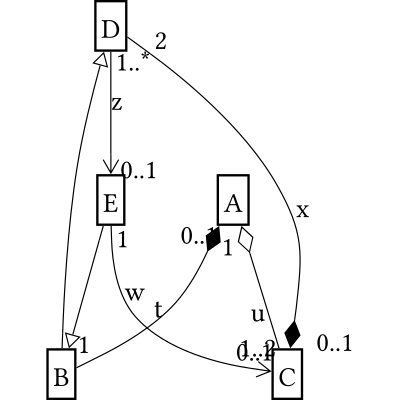
\includegraphics[min width=0.5\textwidth,min height=0.4\textwidth,max width=\textwidth,max height=\textwidth]{58/cd934dbe54d5129f525ee6b192bdbd37ad093629f314be3e5acf67915c2a4cdbc111af83b04c596701db35357ce8aed00a3a92e08161.pdf}}}\figureSeriesRow{\figureSeriesElement{2}{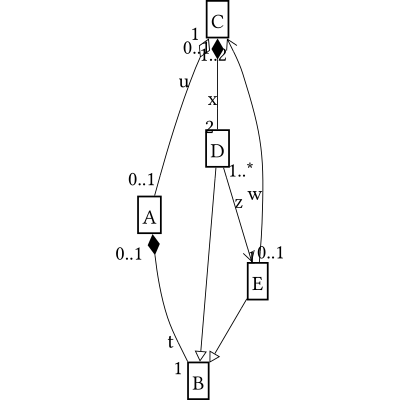
\includegraphics[min width=0.5\textwidth,min height=0.4\textwidth,max width=\textwidth,max height=\textwidth]{58/cde94cdffa7470890fe6b15018df7341d1fb18344e7db340c637d49f0daa8dda8f11af83b04c596701db35357ce8aed00a3a92e08161.pdf}}}}Welche der folgenden fünf Objektdiagramme passen zu welchem Klassendiagramm? 
 Ein Objektdiagramm kann zu keinem, einem oder beiden Klassendiagrammen passen.

\figureSeriesHere{}{\figureSeriesRow{\figureSeriesElement{a}{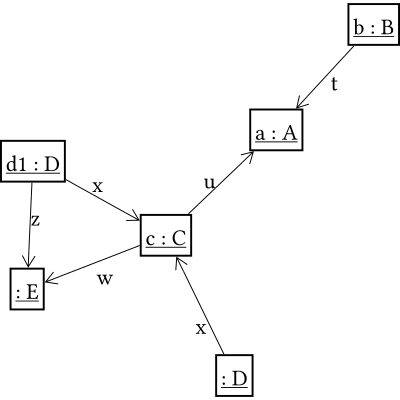
\includegraphics[min width=0.5\textwidth,min height=0.4\textwidth,max width=\textwidth,max height=\textwidth]{58/od2eeeb6dca43e8363240c473a1dbb35ea1f0a44fb90e19038ba38e4fb0c97900810.pdf}}}\figureSeriesRow{\figureSeriesElement{b}{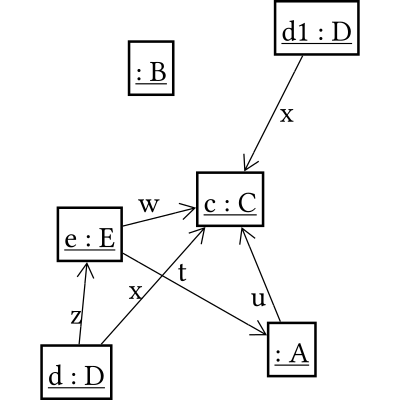
\includegraphics[min width=0.5\textwidth,min height=0.4\textwidth,max width=\textwidth,max height=\textwidth]{58/od255bef62a102504988d71033c07c903b8e23fb81358d2d24b1e78866cd54d9e410.pdf}}}\figureSeriesRow{\figureSeriesElement{c}{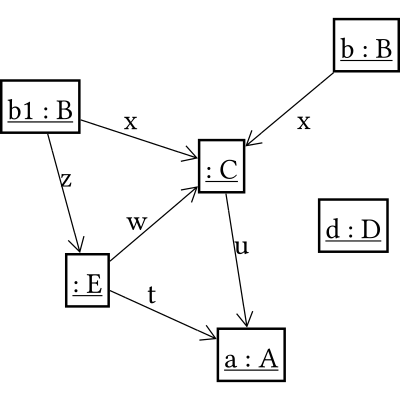
\includegraphics[min width=0.5\textwidth,min height=0.4\textwidth,max width=\textwidth,max height=\textwidth]{58/od0a1961ec2882b393c164f54b1d9beaff252ad85fcf623954f9d3b9130925f70910.pdf}}}\figureSeriesRow{\figureSeriesElement{d}{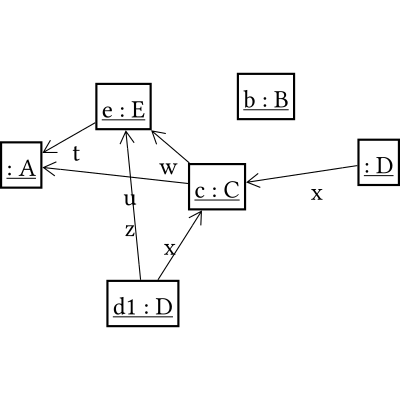
\includegraphics[min width=0.5\textwidth,min height=0.4\textwidth,max width=\textwidth,max height=\textwidth]{58/od8b575725d7aaf2374118b318e2b49b0b78ca7a58b1db5c10461b36fc21441f8a10.pdf}}}\figureSeriesRow{\figureSeriesElement{e}{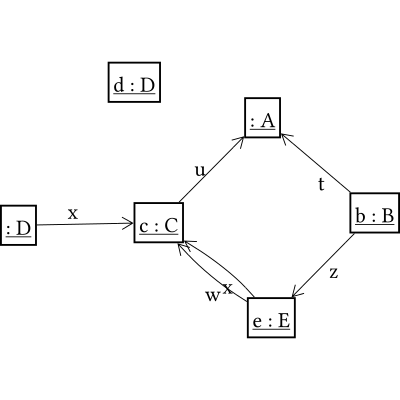
\includegraphics[min width=0.5\textwidth,min height=0.4\textwidth,max width=\textwidth,max height=\textwidth]{58/odd9f84d7d7a3fdce9f56deceecc4ea66712e389524992517940422b1375f6befc10.pdf}}}}Bitte geben Sie Ihre Antwort in Form einer Liste von Paaren an, die jeweils aus einer Klassendiagrammnummer und aus Objektdiagrammbuchstaben bestehen. 
 Jedes Paar gibt an, dass die genannten Objektdiagramme zu dem jeweiligen Klassendiagramm passen. 
 Zum Beispiel drückt 
\begin{minted}{text}
[(1,ab),(2,)]
\end{minted}
aus, dass unter den angebotenen Auswahlmöglichkeiten genau die Objektdiagramme a und b Instanzen des Klassendiagramms 1 sind und dass keines der angebotenen Objektdiagramme Instanz des Klassendiagramms 2 ist.

Bitte beachten Sie: Klassen werden hier vereinfacht dargestellt. 
 Das heißt, sie bestehen aus einer einfachen Box, die nur den Klassennamen enthält, aber keine Abschnitte für Attribute oder Methoden. 
 Trotzdem sollten Sie diese vereinfachten Klassendarstellungen als valide Klassen ansehen.

Da Navigationsrichtungen verwendet werden, beachten Sie bitte, dass Aggregationen und Kompositionen nur vom \glqq{}Teil\grqq{} zum \glqq{}Ganzen\grqq{} navigierbar sind, d.h., sie sind nicht in der entgegengesetzten Richtung navigierbar!

Bitte beachten Sie: Beim Bewegen über oder Klicken auf Kanten / Knoten bzw. ihre Beschriftungen werden die jeweils zusammengehörenden Komponenten hervorgehoben.

